\begin{figure}[h!]
    \centering
    \caption{Estimated landlord shares and counterfactual increases in log rents
            and log total wages, ZIP codes in the Chicago-Naperville-Elgin CBSA}
    \label{fig:map_chicago_cf_rents_wages_shares}

    \begin{subfigure}{.5\textwidth}
        \caption*{Landlord share}
        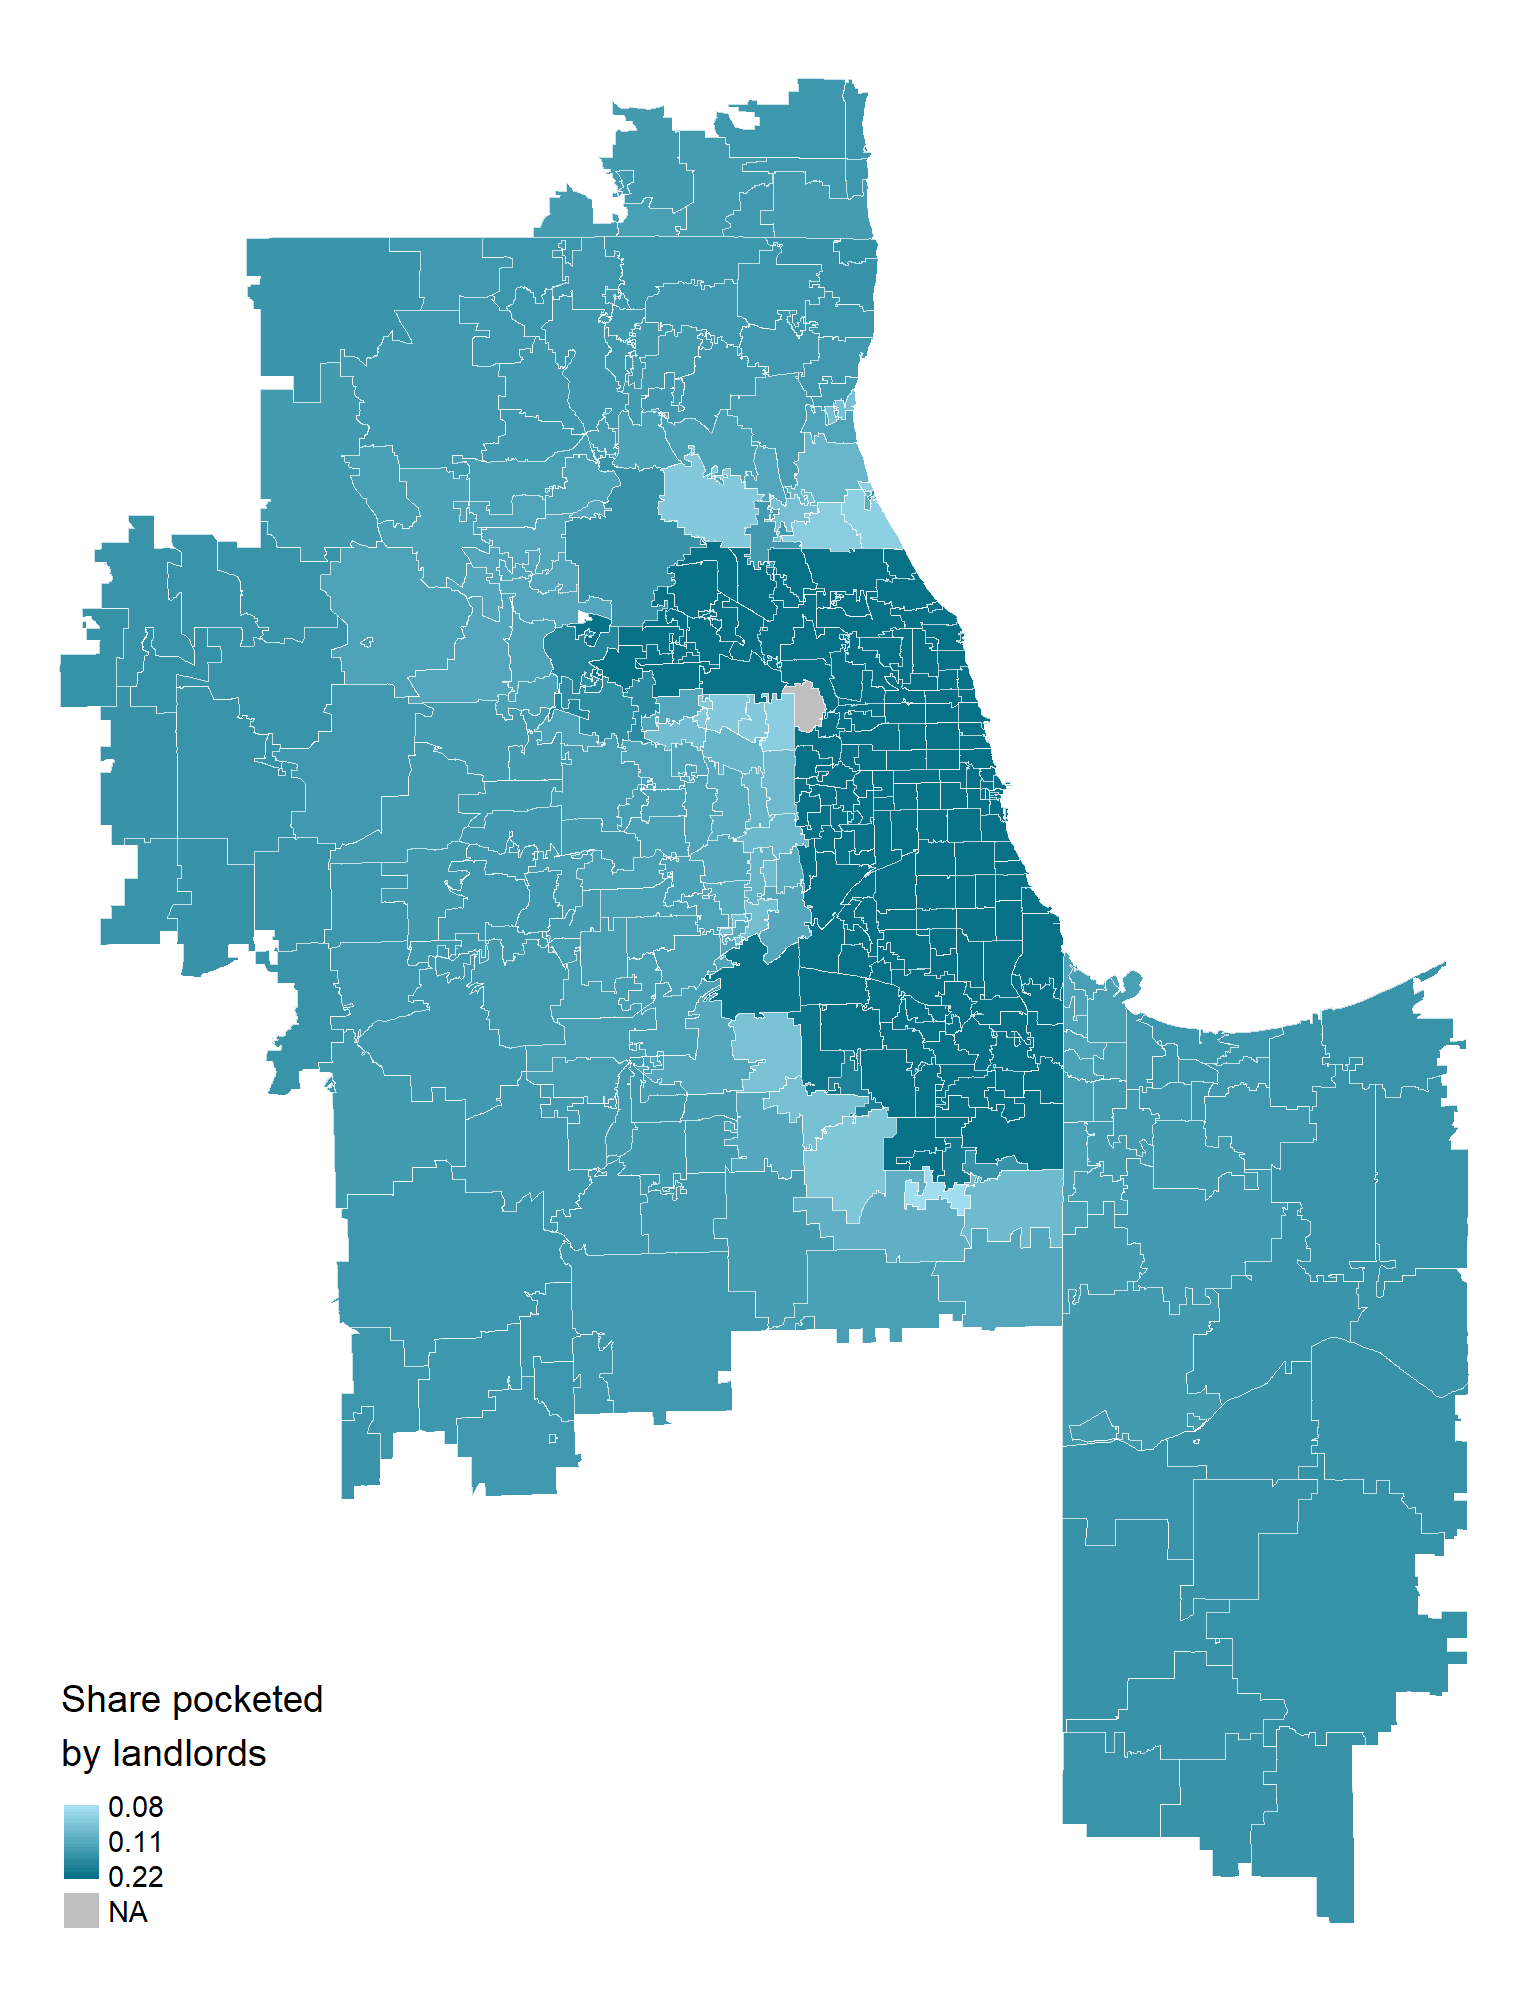
\includegraphics[width = 1\textwidth]
            {counterfactuals/output/chicago_rho.png}
    \end{subfigure}\\
    \begin{subfigure}{.35\textwidth}
        \caption*{Changes in log rents}
        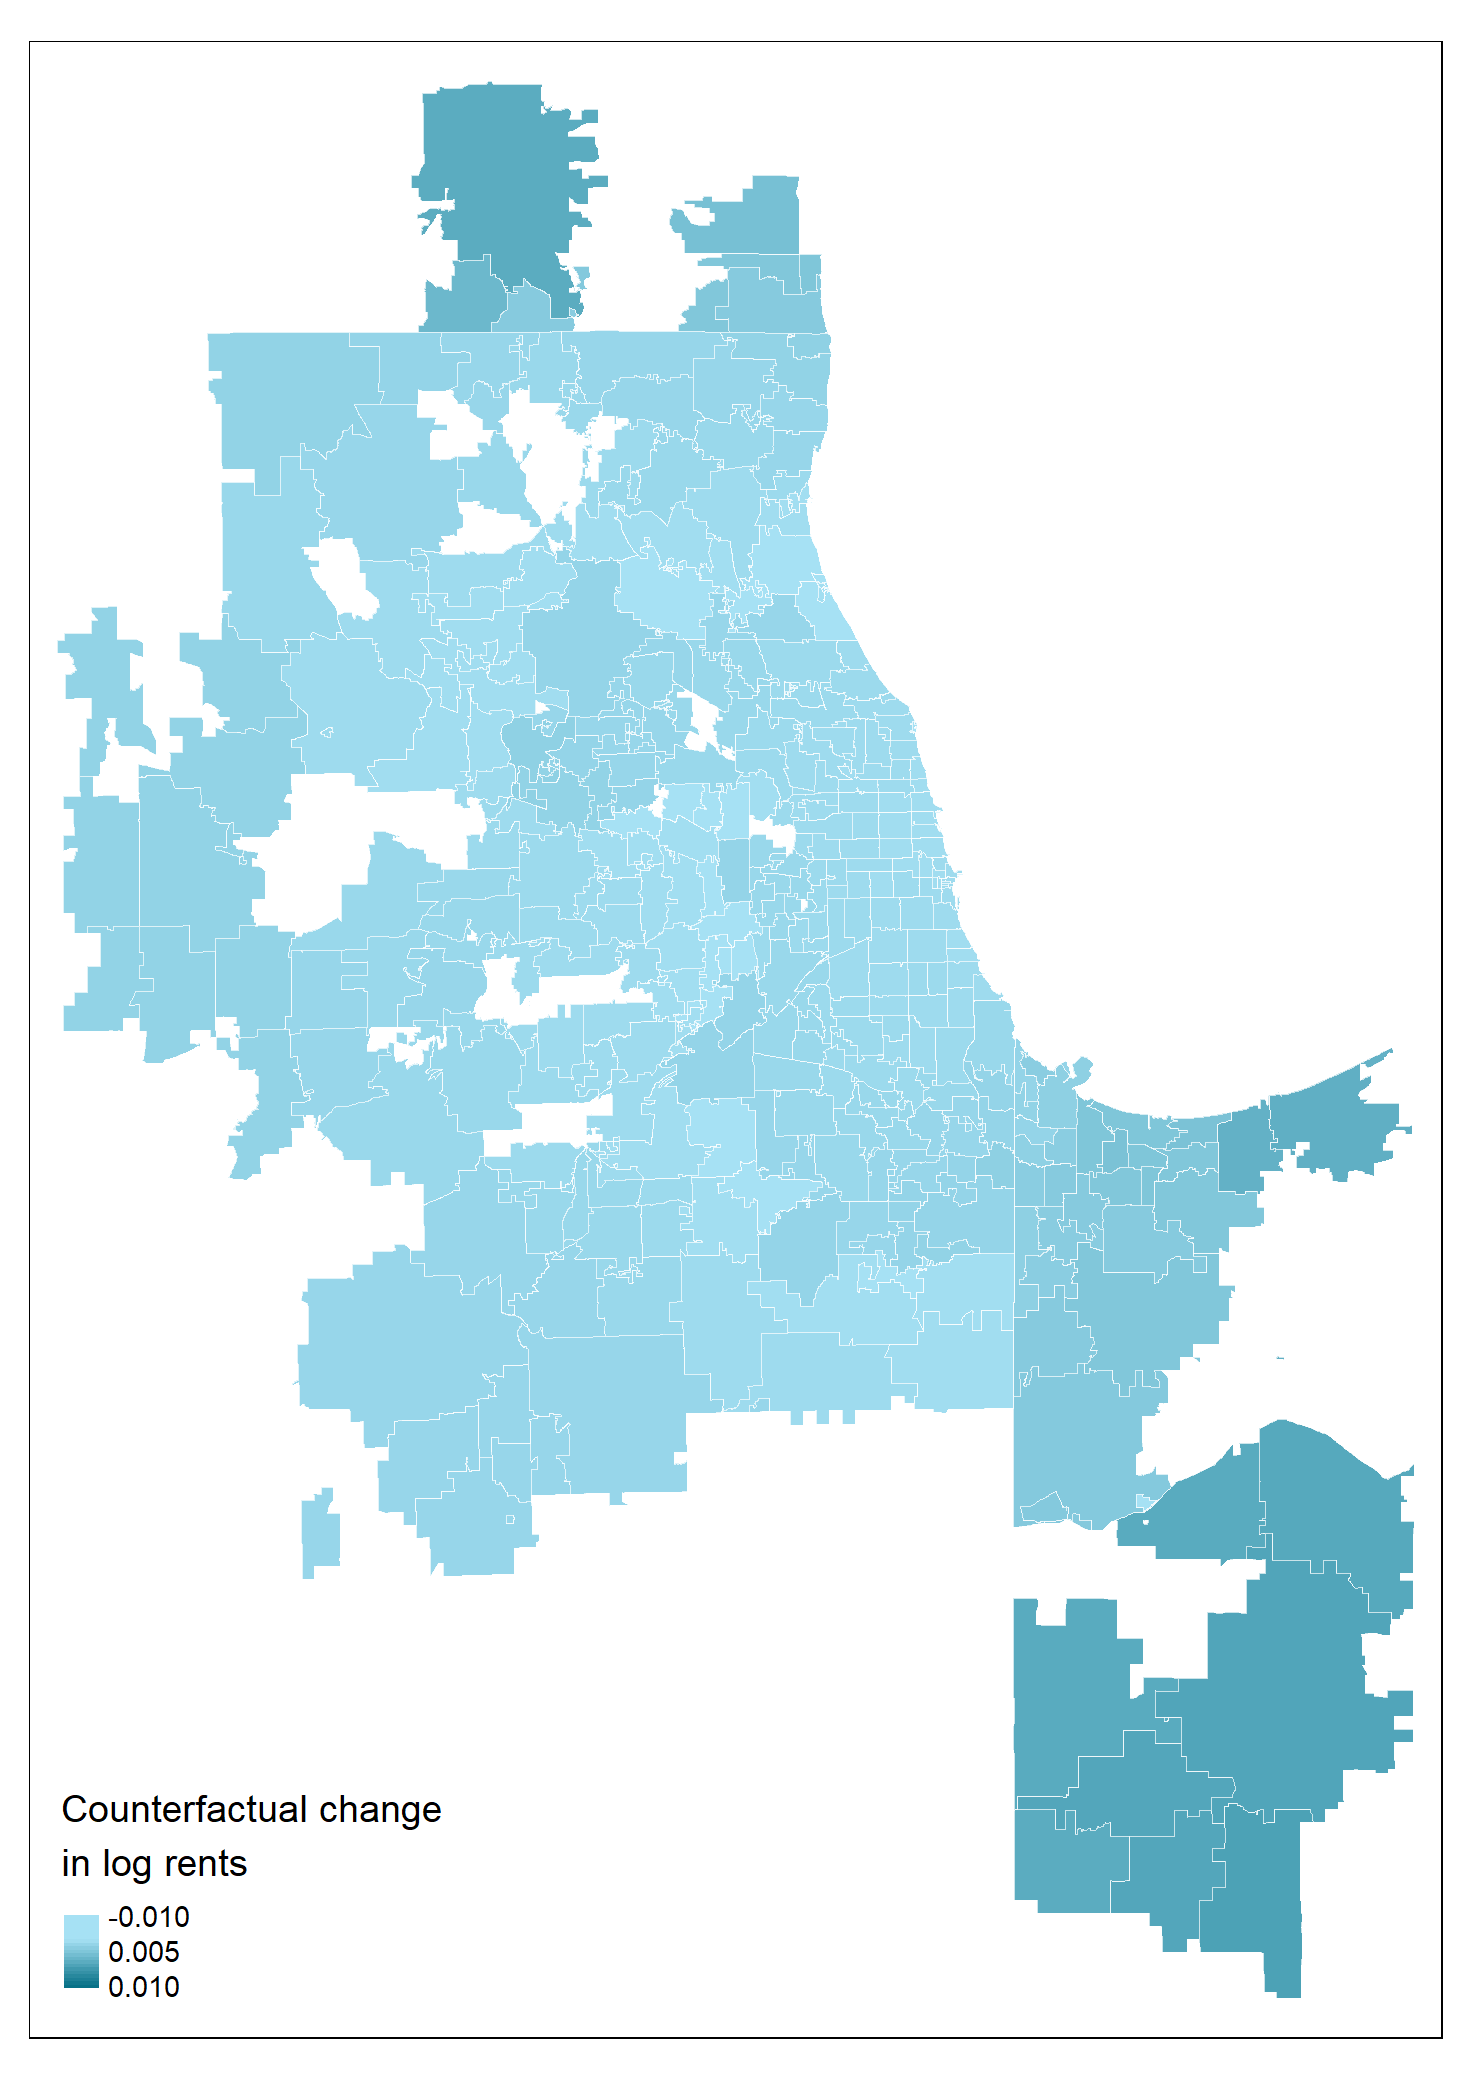
\includegraphics[width = 1\textwidth]
            {counterfactuals/output/chicago_d_ln_rents.png}
    \end{subfigure}%
    \begin{subfigure}{.35\textwidth}
        \caption*{Changes in log total wages}
        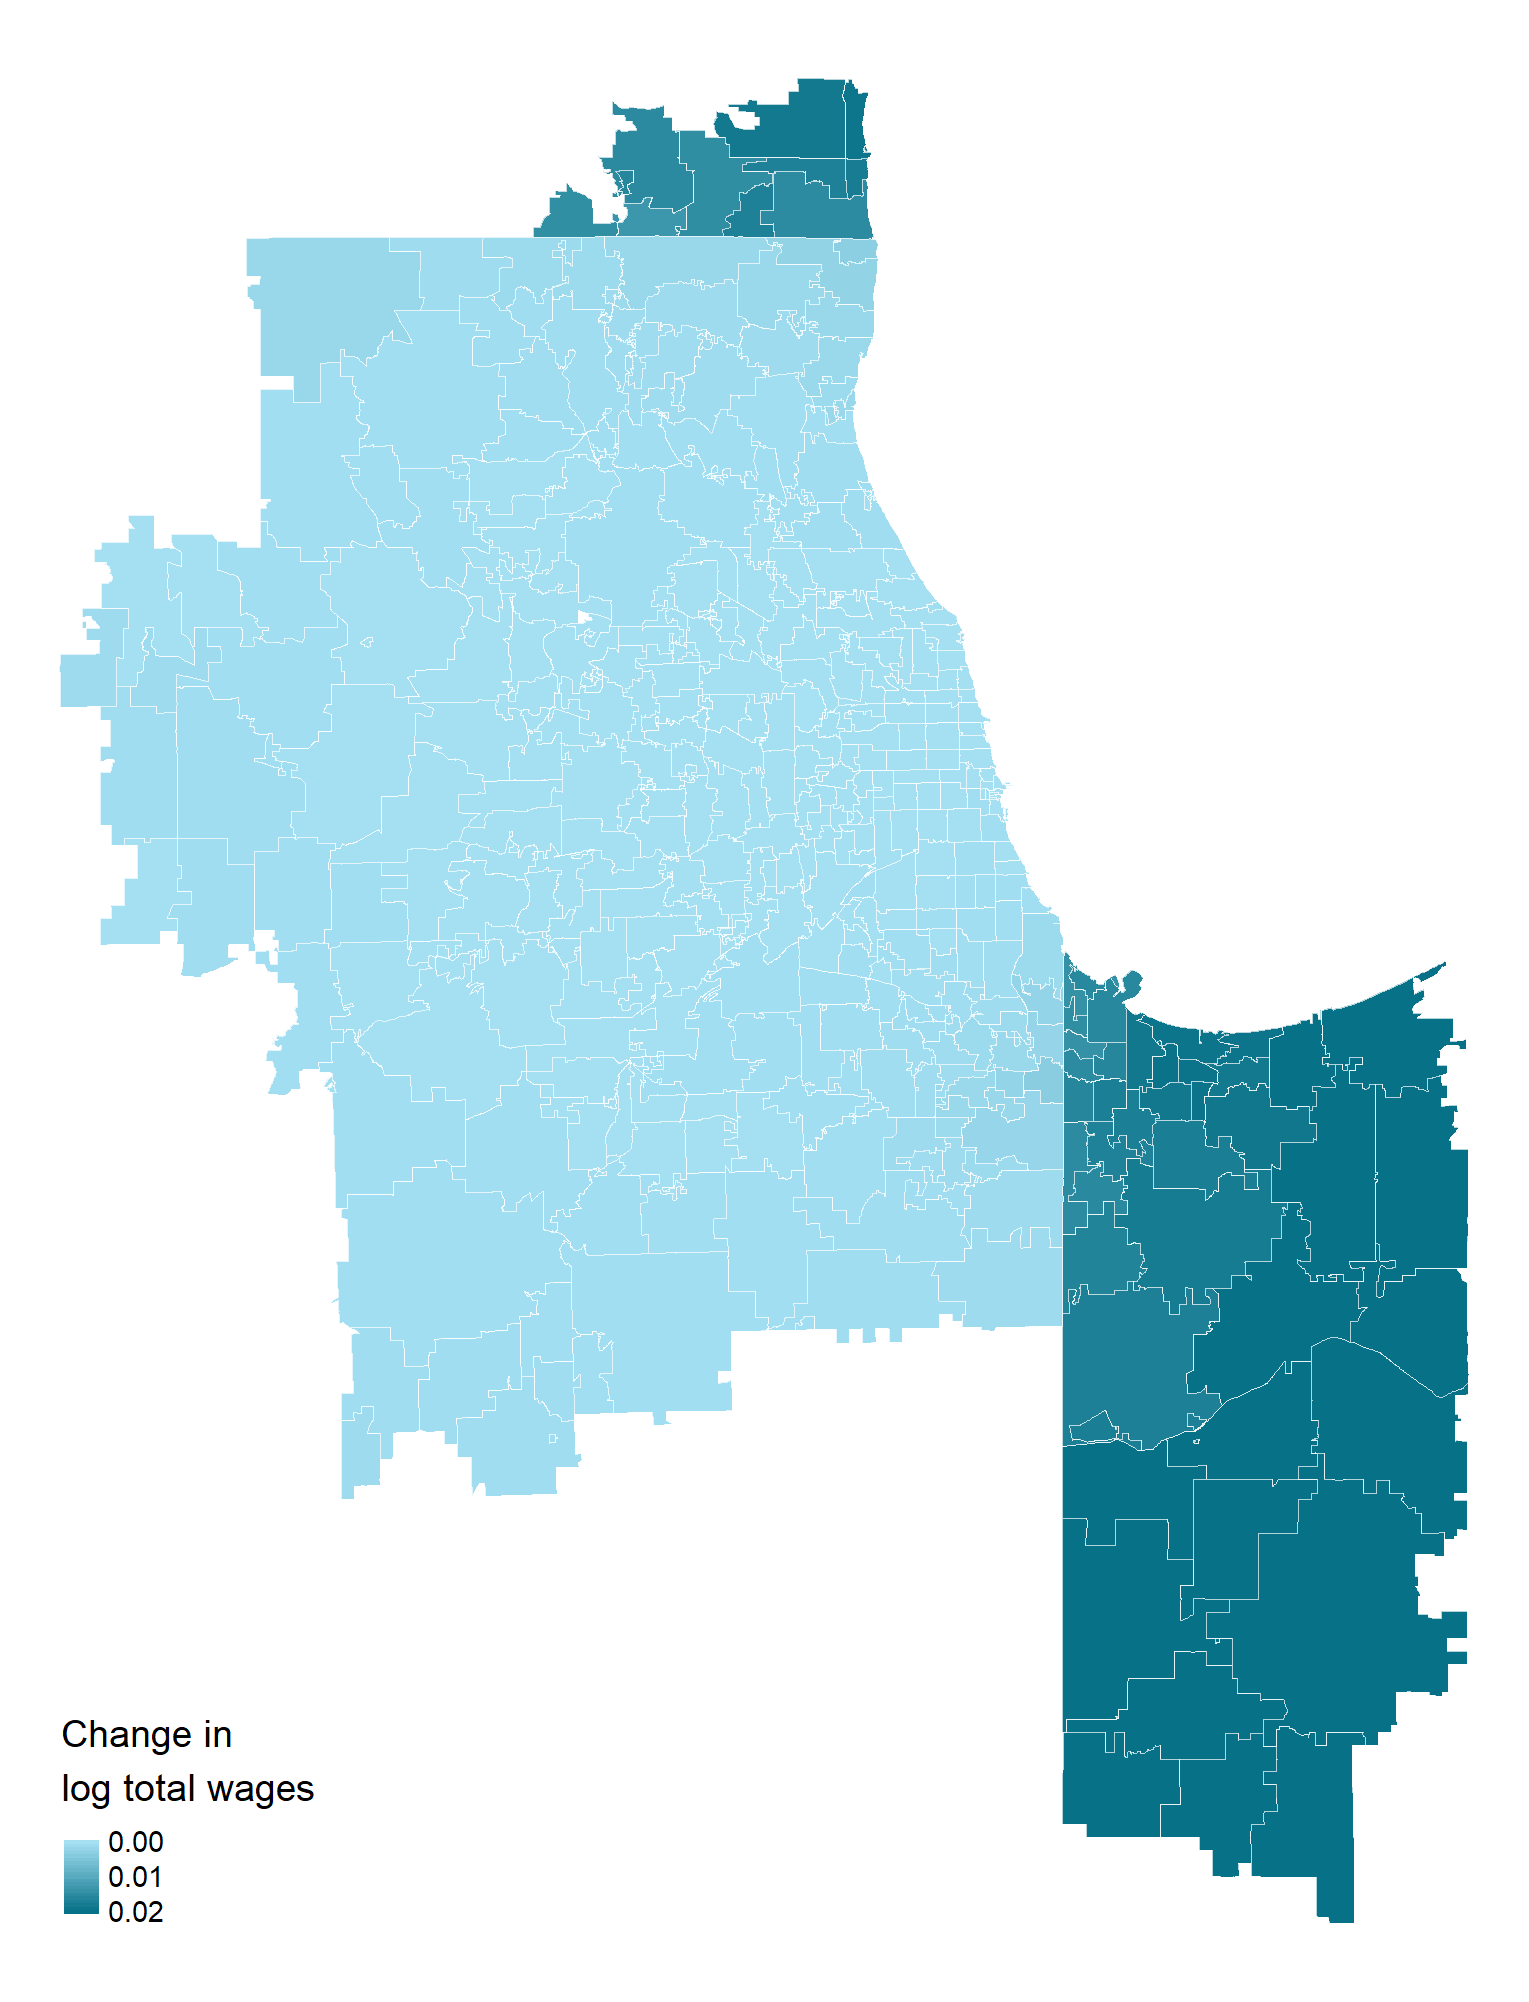
\includegraphics[width = 1\textwidth]
            {counterfactuals/output/chicago_d_ln_wagebill.png}
    \end{subfigure}

    \begin{minipage}{.95\textwidth} \footnotesize
        \vspace{3mm}
        Notes: 
        Data are from LODES and the minimum wage panel described in Section 
        \ref{sec:mw_construction}.
        The top figures maps the distribution of estimated landlord shares, 
        the bottom left figure maps estimated changes in log rents, and 
        the bottom right figure maps estimated changes in log total wages,
        for ZIP codes in the Chicago-Naperville-Elgin CBSA.
        The computations are based on a counterfactual increase to \$9 in the 
        federal MW in January 2020, holding constant other MW policies in their 
        December 2019 levels.
        The landlord share is defined as the ratio between the percent increase 
        in rents and the percent increase in total wages multipled by the share 
        of housing expenditure in the ZIP code.
        To estimate it we follow the procedure described in Section 
        \ref{sec:counterfactual}, assuming the following parameter values: 
        $\beta = 0.0546$, $\gamma = -0.0207$, $\varepsilon = 0.1083$, and 
        $s = 0.35$.
    \end{minipage}
\end{figure}
